%% Creator: Inkscape 0.48.5, www.inkscape.org
%% PDF/EPS/PS + LaTeX output extension by Johan Engelen, 2010
%% Accompanies image file 'everyonesAccuraciesOVERALL0.pdf' (pdf, eps, ps)
%%
%% To include the image in your LaTeX document, write
%%   \input{<filename>.pdf_tex}
%%  instead of
%%   \includegraphics{<filename>.pdf}
%% To scale the image, write
%%   \def\svgwidth{<desired width>}
%%   \input{<filename>.pdf_tex}
%%  instead of
%%   \includegraphics[width=<desired width>]{<filename>.pdf}
%%
%% Images with a different path to the parent latex file can
%% be accessed with the `import' package (which may need to be
%% installed) using
%%   \usepackage{import}
%% in the preamble, and then including the image with
%%   \import{<path to file>}{<filename>.pdf_tex}
%% Alternatively, one can specify
%%   \graphicspath{{<path to file>/}}
%% 
%% For more information, please see info/svg-inkscape on CTAN:
%%   http://tug.ctan.org/tex-archive/info/svg-inkscape
%%
\begingroup%
  \makeatletter%
  \providecommand\color[2][]{%
    \errmessage{(Inkscape) Color is used for the text in Inkscape, but the package 'color.sty' is not loaded}%
    \renewcommand\color[2][]{}%
  }%
  \providecommand\transparent[1]{%
    \errmessage{(Inkscape) Transparency is used (non-zero) for the text in Inkscape, but the package 'transparent.sty' is not loaded}%
    \renewcommand\transparent[1]{}%
  }%
  \providecommand\rotatebox[2]{#2}%
  \ifx\svgwidth\undefined%
    \setlength{\unitlength}{640bp}%
    \ifx\svgscale\undefined%
      \relax%
    \else%
      \setlength{\unitlength}{\unitlength * \real{\svgscale}}%
    \fi%
  \else%
    \setlength{\unitlength}{\svgwidth}%
  \fi%
  \global\let\svgwidth\undefined%
  \global\let\svgscale\undefined%
  \makeatother%
  \begin{picture}(1,0.75)%
    \put(0,0){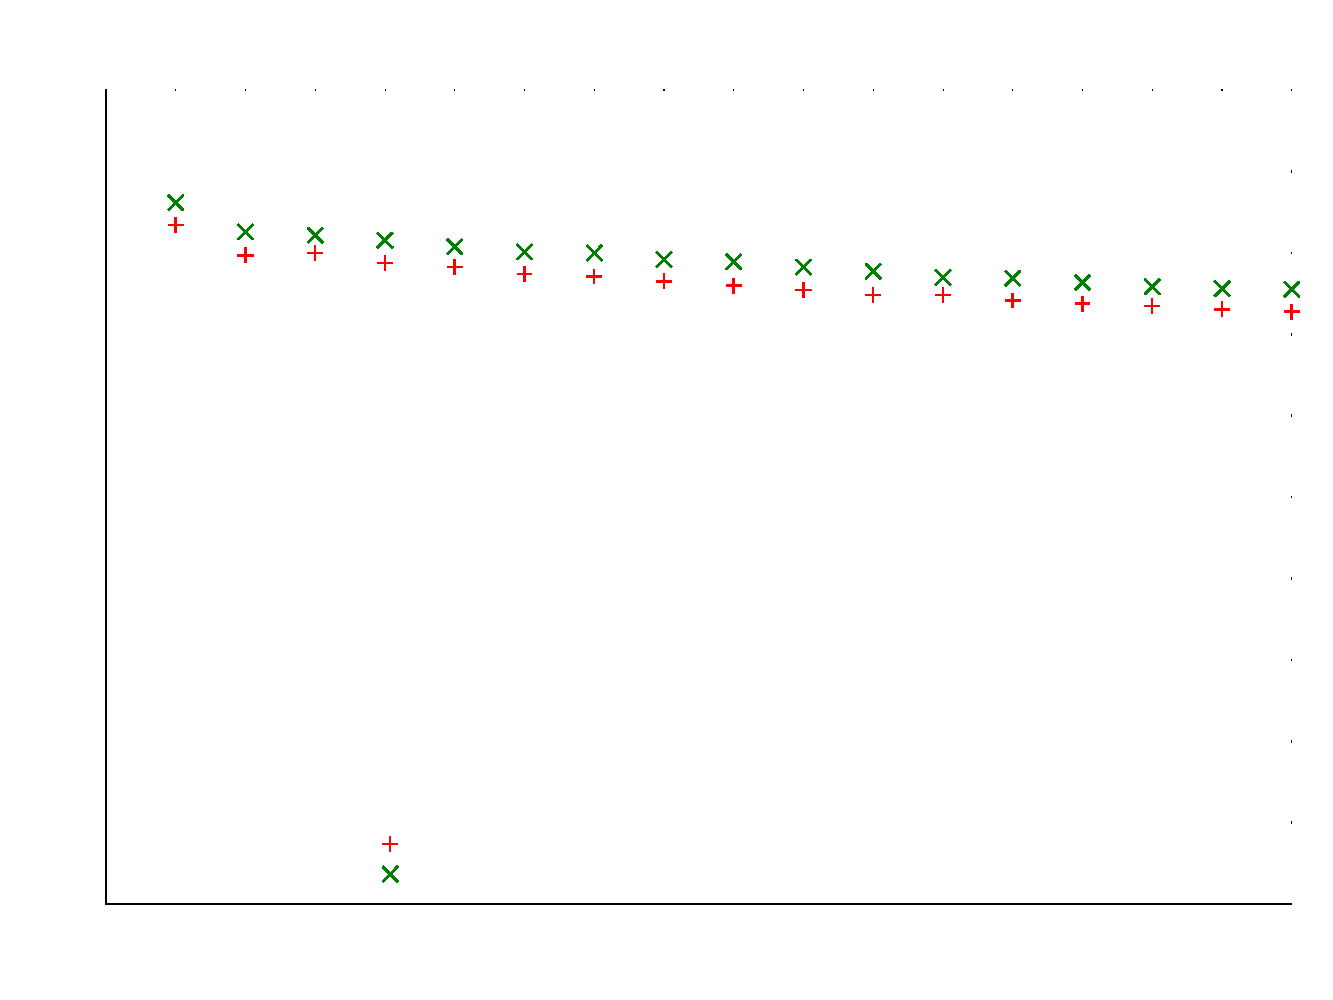
\includegraphics[width=\unitlength]{everyonesAccuraciesOVERALL0.pdf}}%
    \put(0.069125,0.066375){\makebox(0,0)[rb]{\smash{0}}}%
    \put(0.069125,0.127375){\makebox(0,0)[rb]{\smash{10}}}%
    \put(0.069125,0.1885){\makebox(0,0)[rb]{\smash{20}}}%
    \put(0.069125,0.2495){\makebox(0,0)[rb]{\smash{30}}}%
    \put(0.069125,0.3105){\makebox(0,0)[rb]{\smash{40}}}%
    \put(0.069125,0.371625){\makebox(0,0)[rb]{\smash{50}}}%
    \put(0.069125,0.432625){\makebox(0,0)[rb]{\smash{60}}}%
    \put(0.069125,0.493625){\makebox(0,0)[rb]{\smash{70}}}%
    \put(0.069125,0.554625){\makebox(0,0)[rb]{\smash{80}}}%
    \put(0.069125,0.61575){\makebox(0,0)[rb]{\smash{90}}}%
    \put(0.069125,0.67675){\makebox(0,0)[rb]{\smash{100}}}%
    \put(0.0795,0.043875){\makebox(0,0)[b]{\smash{0}}}%
    \put(0.13175,0.043875){\makebox(0,0)[b]{\smash{1}}}%
    \put(0.184125,0.043875){\makebox(0,0)[b]{\smash{2}}}%
    \put(0.236375,0.043875){\makebox(0,0)[b]{\smash{3}}}%
    \put(0.28875,0.043875){\makebox(0,0)[b]{\smash{4}}}%
    \put(0.341,0.043875){\makebox(0,0)[b]{\smash{5}}}%
    \put(0.393375,0.043875){\makebox(0,0)[b]{\smash{6}}}%
    \put(0.445625,0.043875){\makebox(0,0)[b]{\smash{7}}}%
    \put(0.498,0.043875){\makebox(0,0)[b]{\smash{8}}}%
    \put(0.55025,0.043875){\makebox(0,0)[b]{\smash{9}}}%
    \put(0.602625,0.043875){\makebox(0,0)[b]{\smash{10}}}%
    \put(0.654875,0.043875){\makebox(0,0)[b]{\smash{11}}}%
    \put(0.70725,0.043875){\makebox(0,0)[b]{\smash{12}}}%
    \put(0.7595,0.043875){\makebox(0,0)[b]{\smash{13}}}%
    \put(0.811875,0.043875){\makebox(0,0)[b]{\smash{14}}}%
    \put(0.864125,0.043875){\makebox(0,0)[b]{\smash{15}}}%
    \put(0.9165,0.043875){\makebox(0,0)[b]{\smash{16}}}%
    \put(0.96875,0.043875){\makebox(0,0)[b]{\smash{17}}}%
    \put(0.022,0.377125){\rotatebox{90}{\makebox(0,0)[b]{\smash{Overall Accuracy(%)}}}}%
    \put(0.524125,0.010125){\makebox(0,0)[b]{\smash{k}}}%
    \put(0.524125,0.7105){\makebox(0,0)[b]{\smash{OVERALL Accuracy as $k$ Increases with $\alpha$ Threshold 0.0}}}%
    \put(0.255875,0.111375){\makebox(0,0)[rb]{\smash{OVERALL: 16S-23S}}}%
    \put(0.255875,0.088875){\makebox(0,0)[rb]{\smash{OVERALL: 23S-5S}}}%
  \end{picture}%
\endgroup%
